\documentclass{beamer}

\usepackage{amssymb,amsmath}
\usepackage{graphicx}
\usepackage{url}
\usepackage{color}
\usepackage{relsize}		% For \smaller
\usepackage{url}			% For \url
\usepackage{epstopdf}	% Included EPS files automatically converted to PDF to include with pdflatex
\usepackage{pagenote}[continuous,page]

%For MindMaps
% \usepackage{tikz}%
% \usetikzlibrary{mindmap,trees,arrows}%

%%% Color Definitions %%%%%%%%%%%%%%%%%%%%%%%%%%%%%%%%%%%%%%%%%%%%%%%%%%%%%%%%%
%\definecolor{bordercol}{RGB}{40,40,40}
%\definecolor{headercol1}{RGB}{186,215,230}
%\definecolor{headercol2}{RGB}{80,80,80}
%\definecolor{headerfontcol}{RGB}{0,0,0}
%\definecolor{boxcolor}{RGB}{186,215,230}

%%% Save space in lists. Use this after the opening of the list %%%%%%%%%%%%%%%%
%\newcommand{\compresslist}{
%	\setlength{\itemsep}{1pt}
%	\setlength{\parskip}{0pt}
%	\setlength{\parsep}{0pt}
%}

%\setbeameroption{show notes on top}

% You should run 'pdflatex' TWICE, because of TOC issues.

% Rename this file.  A common temptation for first-time slide makers
% is to name it something like ``my_talk.tex'' or
% ``john_doe_talk.tex'' or even ``discrete_math_seminar_talk.tex''.
% You really won't like any of these titles the second time you give a
% talk.  Try naming your tex file something more descriptive, like
% ``riemann_hypothesis_short_proof_talk.tex''.  Even better (in case
% you recycle 99% of a talk, but still want to change a little, and
% retain copies of each), how about
% ``riemann_hypothesis_short_proof_MIT-Colloquium.2000-01-01.tex''?

\mode<presentation>
{
  % A tip: pick a theme you like first, and THEN modify the color theme, and then add math content.
  % Warsaw is the theme selected by default in Beamer's installation sample files.

  %%%%%%%%%%%%%%%%%%%%%%%%%%%% THEME
  %\usetheme{Madrid}		% No subsection
  \usetheme{AnnArbor}  % Subsection on top, no color


  %\usetheme{Antibes}
  %\usetheme{Bergen}
  %\usetheme{Berkeley}		% bem bacana - menu esquerdo
  %\usetheme{Berlin}
  %\usetheme{Boadilla}
  %\usetheme{boxes}
  %\usetheme{CambridgeUS}		% bem bacana - menu superior
  %\usetheme{Copenhagen}
  %\usetheme{Darmstadt}
  %\usetheme{default}
  %\usetheme{Dresden}
  %\usetheme{Frankfurt}
  %\usetheme{Goettingen}
  %\usetheme{Hannover}		% bem bacana - menu esquerdo
  %\usetheme{Ilmenau}
  %\usetheme{JuanLesPins}
  %\usetheme{Luebeck}
  %\usetheme{Malmoe}
  %\usetheme{Marburg}		% bem bacana - menu direito
  %\usetheme{Montpellier}
  %\usetheme{PaloAlto}		% bem bacana - menu esquerdo
  %\usetheme{Pittsburgh}
  %\usetheme{Rochester}		%bacana
  %\usetheme{Singapore}
  %\usetheme{Szeged}
  %\usetheme{Warsaw}

  %%%%%%%%%%%%%%%%%%%%%%%%%%%% COLOR THEME
  %\usecolortheme{default}		% branco, azul clarinho
  \usecolortheme{crane}		% Very yellow (ok)

  %\usecolortheme{albatross}		% azul escuro, massa
  %\usecolortheme{beetle}		% cinza, menu azul
  %\usecolortheme{dolphin}		% azul e branco, legal
  %\usecolortheme{dove}			% cinza e branco, feio
  %\usecolortheme{fly}			% todo cinza, horrível
  %\usecolortheme{lily}			% parece o default
  %\usecolortheme{orchid}		% azul e branco, ok
  %\usecolortheme{rose}			% branco e violeta-claro, bonito
  %\usecolortheme{seagull}		% cinza, feio
  %\usecolortheme{seahorse}		% nhé, meio feio
  %\usecolortheme{sidebartab}		% Azul, branco, destaque na tab, interessante
  %\usecolortheme{structure}		% bichado
  %\usecolortheme{whale}		% Azul e branco, bem bonito

  %%%%%%%%%%%%%%%%%%%%%%%%%%%% OUTER THEME
  \useoutertheme{default}
  %\useoutertheme{infolines}
  %\useoutertheme{miniframes}
  %\useoutertheme{shadow}
  %\useoutertheme{sidebar}
  %\useoutertheme{smoothbars}
  %\useoutertheme{smoothtree}
  %\useoutertheme{split}
  %\useoutertheme{tree}

  %%%%%%%%%%%%%%%%%%%%%%%%%%%% INNER THEME
  \useinnertheme{circles}
  %\useinnertheme{default}
  %\useinnertheme{inmargin}
  %\useinnertheme{rectangles}
  %\useinnertheme{rounded}

  %%%%%%%%%%%%%%%%%%%%%%%%%%%%%%%%%%%

  \setbeamercovered{invisible} % or whatever (possibly just delete it)
  % To change behavior of \uncover from graying out to totally
  % invisible, can change \setbeamercovered to invisible instead of
  % transparent. apparently there are also 'dynamic' modes that make
  % the amount of graying depend on how long it'll take until the
  % thing is uncovered.

}


% Get rid of nav bar
\beamertemplatenavigationsymbolsempty

% Use short top
%\usepackage[headheight=12pt,footheight=12pt]{beamerthemeboxes}
%\addheadboxtemplate{\color{black}}{
%\hskip0.5cm
%\color{white}
%\insertshortauthor \ \ \ \
%\insertframenumber \ \ \ \ \ \ \
%\insertsection \ \ \ \ \ \ \ \ \ \ \ \ \ \ \ \ \  \insertsubsection
%\hskip0.5cm}
%\addheadboxtemplate{\color{black}}{
%\color{white}
%\ \ \ \
%\insertsection
%}
%\addheadboxtemplate{\color{black}}{
%\color{white}
%\ \ \ \
%\insertsubsection
%}

% Insert frame number at bottom of the page.
% \usefoottemplate{\hfil\tiny{\color{black!90}\insertframenumber}}

%% makes the ppagenote command for figure references at the end.

\usepackage[english]{babel}
%qq\usepackage[latin1]{inputenc}
\usepackage{CJKutf8}
\usepackage{subfigure}

\usepackage{times}
\usepackage[T1]{fontenc}

\makepagenote
\renewcommand{\notenumintext}[1]{}
\newcommand{\ppagenote}[1]{\pagenote[Page \insertframenumber]{#1}}

\title[Programming Challenges]{GB20602 - Programming Challenges}
\author[Claus Aranha]{Claus Aranha\\{\footnotesize caranha@cs.tsukuba.ac.jp}}
\institute[U. Tsukuba]{University of Tsukuba, Department of Computer Sciences}


\title[GB21802]{GB21802 - Programming Challenges}
\subtitle[]{Week 1 - Basic Problem Solving}
\author[Claus Aranha]{Claus Aranha\\{\footnotesize caranha@cs.tsukuba.ac.jp}}
\institute{College of Information Science}
\date{2015-04-13\\{\tiny Last updated \today}}

\begin{document}

\section{Prologue}
\subsection{Title}
\begin{frame}
\maketitle
\end{frame}

\subsection{Notes and Warnings}

\begin{frame}
  \frametitle{Some Notes Before the Class}
  \begin{exampleblock}{Please check your ``Programming Challenge'' username!}
    Some people submitted me invalid usernames:
    \begin{itemize}
    \item ``Oda''
    \item ``dai''
    \end{itemize}
    Everyone, please don't forget to send your usernames!
  \end{exampleblock}
  \vfill
  \begin{exampleblock}{Early submissions}
    We already had some early submissions -- fantastic!
    \medskip
    Any problems or questions regarding the submission proccess?
  \end{exampleblock}
\end{frame}

\begin{frame}
  \frametitle{Summary for Last Class}
  \begin{exampleblock}{How the course works}
    \begin{itemize}
      {\smaller
    \item Monday Class: Theme exposition;
    \item Friday Class: Example problem and Q\&A;
    \item Problems: Solve 4 problems every week;
      }
    \end{itemize}
  \end{exampleblock}
  \begin{exampleblock}{How to submit the problems}
    {\smaller
    \begin{itemize}
    \item Make an account at \url{www.programming-challenges.com}
    \item Send your username to the professor (manaba or e-mail)
    \item Write the program in C, C++, Java or Pascal
    \end{itemize}}
  \end{exampleblock}
  \begin{exampleblock}{How evaluation works}
    {\smaller
    \begin{itemize}
    \item Grade = number of problems submitted
    \item Try to submit one problem per week
    \item Comments and Participation counts
    \end{itemize}}
  \end{exampleblock}
  
\end{frame}

\begin{frame}
  \frametitle{Summary for This Class}
  \begin{description}
    \item[General Problem Solving]:\\ A very important skill which is hard to teach formally;
      \vspace{.5cm}
    \item[Data Structures and Programming Challenges]:\\ How to think of
      data structures outside of the classroom;
      \vspace{.5cm}
    \item[Problem Discussion]:\\ Let's introduce last week's problems;
  \end{description}

  \begin{exampleblock}{Relax, and ask questions!}
    No topic here is really new. Listen carefully!
    
    \bigskip
    
    Ask questions any time!
  \end{exampleblock}
\end{frame}

%%%%%%%%%%%%%%%%%%%%%%%%%%%%%%%%%%%%%%%%%%%%%%%%%%%%%%%%%

\section{Problem Solving}
\subsection{What is problem solving skill?}

\begin{frame}
  \begin{center}
    {\bf Problem Solving Skills}
  \end{center}
\end{frame}

\begin{frame}
  \frametitle{What are problem solving skills? (1)}
  
  \begin{columns}
    \column{0.3\textwidth}
    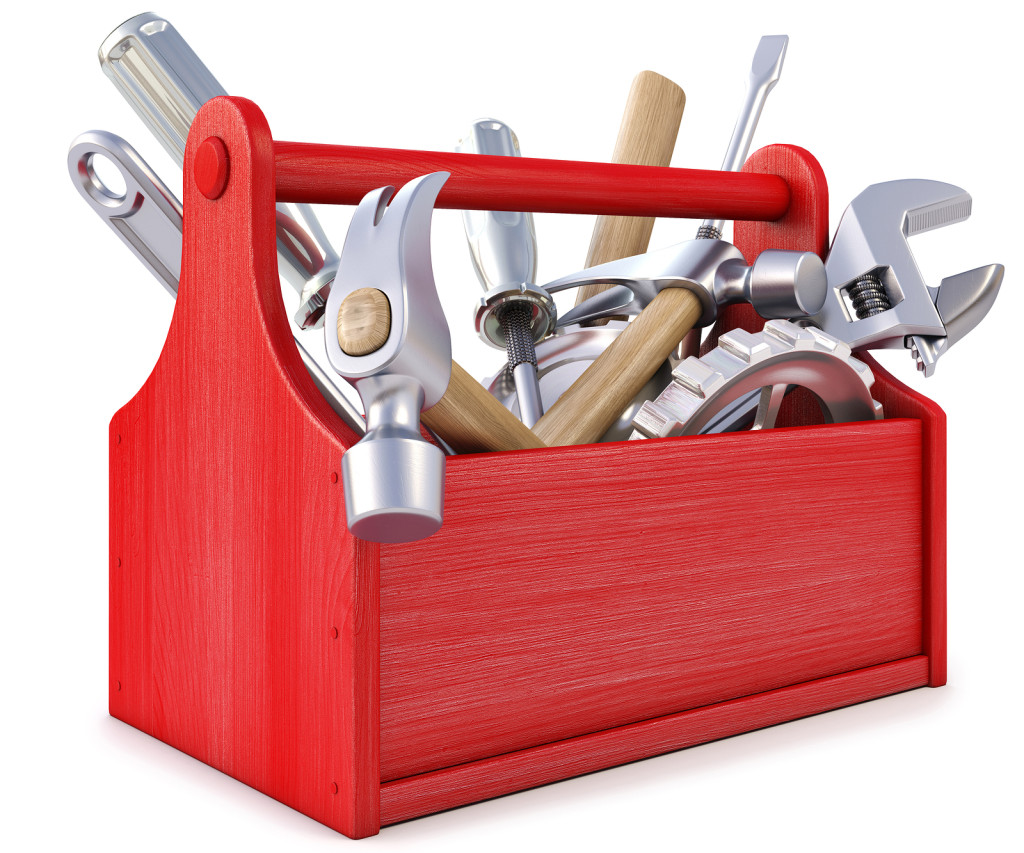
\includegraphics[width=1\textwidth]{img/toolbox}
    \column{0.7\textwidth} 
    I'm sure you are all very good programmers. You all know many
    techniques.
  \end{columns}

  \medskip

  \begin{itemize}
    \item Data Structures
    \item Languages and Libraries
    \item Sorting Algorithms
    \item Script Tools
    \item Etc...
  \end{itemize}
  
  \begin{center}
    But choosing the right technique for a problem is a \alert{hard}
    skill.
  \end{center}
  
\end{frame}

\begin{frame}
  \frametitle{What are problem solving skills? (2)}
  \begin{columns}[T]
    \column{0.6\textwidth}
    
    {\small
    Some people don't know what method to solve a problem, unless they
    are told.} 

    \vspace{0.5cm}
    
    {\small
    Other people always use their favorite technique, no matter what
    is the problem.}
    
    \vspace{0.5cm}

    \begin{center}
      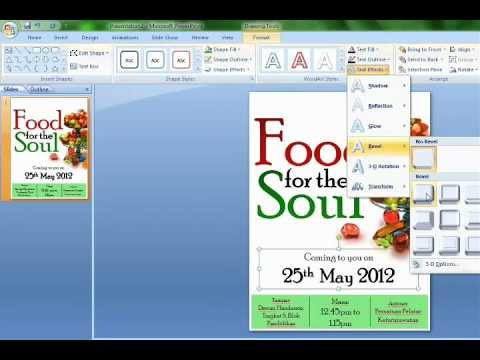
\includegraphics[width=0.8\textwidth]{img/powerpoint}
    \end{center}
    \column{0.4\textwidth}
    
\includegraphics[height=0.8\textheight]{img/hammer}
  \end{columns}
\end{frame}

\begin{frame}

  A \structure{Problem} can be solved \structure{Any way} we want. But
  our brains don't like that:

  \begin{exampleblock}{Difficulty 1: Irrelevant Information}
    Problems usually have information that is not necessary. If we
    don't identify this information and erase it, the problem may be
    impossible.
  \end{exampleblock}

  \begin{exampleblock}{Difficulty 2: Functional Fixedness}
    We learn that some tools are for some functions. Sometimes they
    can be used for other goals (for example, glue and paper for a
    message)
  \end{exampleblock}


  \begin{block}{}
    One of the goals of this course is to help you develop
    \structure{Problem Solving Skills}. It will be important for your
    entire life.
  \end{block}
\end{frame}

\subsection{Steps to solve a problem}
\begin{frame}
  \frametitle{Steps to solve a (Programming) problem} 

  Don't know where to begin?  Don't panic, keep calm, and try to
  follow these steps.

  \begin{enumerate}
  \item Read the input and output
  \item Summarize the problem
  \item Check for traps
  \item Write the program
  \item Test/Debug
  \item Submit!
  \end{enumerate}
\end{frame}

\begin{frame}
  \frametitle{Step 1: Input and Output}

  \begin{block}{First read the input and output quickly}
    Reading the desired input and output gives you a general idea of
    what is expected. It helps \structure{put your mind in the right
      mood}.
  \end{block}
  
  \medskip
  
  \begin{itemize}
  \item Are you dealing with integers or floats?
  \item Are strings necessary?
  \item How big is the input?
  \item Is the input ordered?
  \end{itemize}
  
  \begin{block}{}
    ``What does this problem wants from me?''
  \end{block}
\end{frame}

\begin{frame}
  \frametitle{Step 2: Problem Summary}
  
  \begin{block}{Read the entire problem and discover the goal}
    Find out what is the relationship between the \structure{Input}
    and the \structure{Output}.
  \end{block}
  \begin{itemize}
  \item Print out the Problem!
  \item Cross out \alert{irrelevant information}
  \item \alert{Mark down} important information.

    \bigskip
    
  \item Write down an algorithm to solve the problem
  \item Read the problem again
  \item Repeat until you are confident
  \end{itemize}
\end{frame}

\begin{frame}
  \frametitle{Step 3: Problem Traps}
  \begin{columns}[T]
    \column{0.7\textwidth}
    \begin{block}{}
      Read the problem one more time. There are often ``Traps'' in the
      problem description.
    \end{block}
    \column{0.2\textwidth}
    
\includegraphics[width=1\textwidth]{img/ackbar}
  \end{columns}

  \begin{itemize}
    {\small
  \item Does the Problem require rounding off of numbers? (Round Up,
    Round Down, Round to nearest)
  \item Can the input order be reversed? (Big first, Small First, out of order)
  \item What is the maximum size of the input? 100? 10000? 1000000000?
  \item Can the input be negative? Can the input be zero?}
  \end{itemize}
\end{frame}

\begin{frame}
  \frametitle{Problem Trap Example 1}
  \begin{columns}[T]
    \column{0.3\textwidth}
    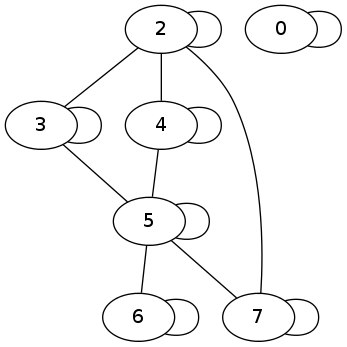
\includegraphics[width=1\textwidth]{img/graph1}    
    \column{0.7\textwidth}
    Graph Problems:
    \begin{itemize}
    \item Does the graph have self-cycles? (search can go in infinite loops)
      \vspace{.5cm}

    \item Is the graph connected? (some nodes are unreachable)
      \vspace{.5cm}

    \item Are all weights positive? (Djikstra does not work)
    \end{itemize}
  \end{columns}
\end{frame}

\begin{frame}
  \frametitle{Problem Trap Example 2}
  \begin{columns}[T]
    \column{0.3\textwidth}
    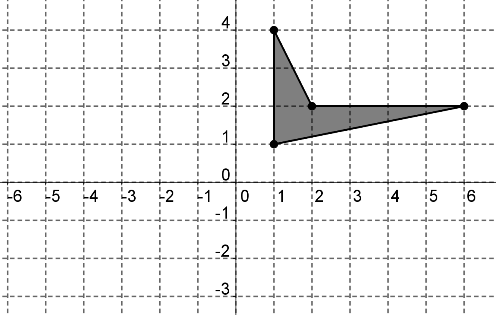
\includegraphics[width=1\textwidth]{img/polygon}    
    \column{0.7\textwidth}
    Geometry Problems:
    \begin{itemize}
    \item Can the polygon be convex? (harder algorithms)
      \vspace{.5cm}

    \item Can two points be in the same place? (division by zero)
      \vspace{.5cm}

    \item Can points have negative coordinates? (multiplication issues)
    \end{itemize}
  \end{columns}
\end{frame}


\subsection{programming}

\begin{frame}
  \frametitle{Step 4: Write the program}

  You should do steps 1, 2 and 3 \alert{on paper}
  \medskip
  \begin{center}
  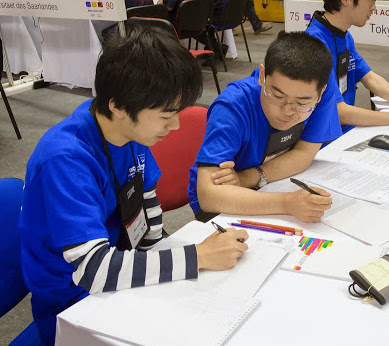
\includegraphics[width=0.5\textwidth]{img/writing}
  \end{center}
  \medskip
  Only start writing the program after you understand your
  solution. (easier to avoid bugs!)
\end{frame}

\begin{frame}
  \frametitle{Step 4: Write the Program (some hints)}

  \begin{block}{Do Input/output first}
    \begin{itemize}
    \item You can't test without IO
    \item Check the end condition: EOF or Special Case?
    \end{itemize}
  \end{block}

  \begin{block}{Test Often}
    \begin{itemize}
    \item Test your program on the test data
    \item Re-test your program every time you do a small change
    \end{itemize}    
  \end{block}
\end{frame}

\begin{frame}
  \frametitle{Step 4: Algorithm Efficiency, Programmer Efficiency}

  \begin{block}{Algorithm Efficiency}
    \begin{itemize}
      \item Pay attention to the size of the input!
      \item Always calculate the complexity of your algorithm,\\
        $O(n), O(n^2), O(n^3)$, etc...
      \item Multiply the complexity by the input size.
    \end{itemize}
  \end{block}

  \begin{block}{Programmer Efficiency}
    \begin{itemize}
    \item Avoid overly complex code!
    \item Double linked lists are very efficient...
    \item ... but they are not necessary if your input size is 100.
    \end{itemize}
  \end{block}
\end{frame}

\begin{frame}
  \frametitle{Step 4: Hints for C/C++}
  \begin{itemize}
  \item Love the stl;
    \vspace {.5 cm}
  \item Avoid messing with pointers;
    \vspace {.5 cm}
  \end{itemize}
\end{frame}

\begin{frame}
  \frametitle{Step 4: Hints for Java}
  \begin{itemize}
  \item Object Oriented programming is great, but not very useful for this lecture;
    \vspace{.5cm}
  \item Abuse java.util:
    \vspace{.5cm}
  \item All classes must be in the same file;
  \end{itemize}
\end{frame}

\begin{frame}
  \frametitle{Step 4: Hints for Pascal}
  \begin{center}
  
\includegraphics[width=0.7\textwidth]{img/pascal}
  \end{center}
\end{frame}

\subsection{Problem solving example}
\begin{frame}
  \begin{center}
    Problem Solving Example: ``The Trip''
  \end{center}
\end{frame}

%%%%%% Week 2 -- Data structures %%%%%%%%%

\section{Data Structures}
\subsection{Introduction}

\begin{frame}
  \begin{center}
    {\bf Data Structures}
  \end{center}
\end{frame}

\begin{frame}
  \frametitle{Data Structures}

  \begin{block}{Data structures are the heart of a program}
    \begin{itemize}
      {\small
      \item Using the correct data type can make a problem much easier;
      \item Using the incorrect data type can make a problem much harder;
      }
    \end{itemize}
  \end{block}

  \begin{block}{The towers of Hanoi}
    \begin{center}
    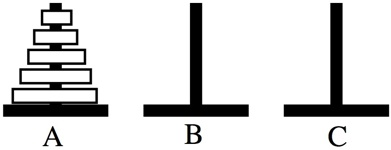
\includegraphics[width=0.5\textwidth]{img/hanoi}
    \end{center}
    \medskip
    QUIZ: How do you represent the data in this problem? 
  \end{block}
\end{frame}

\begin{frame}
  \frametitle{An easy way to visualize the Towers of Hanoi}
  \begin{center}
    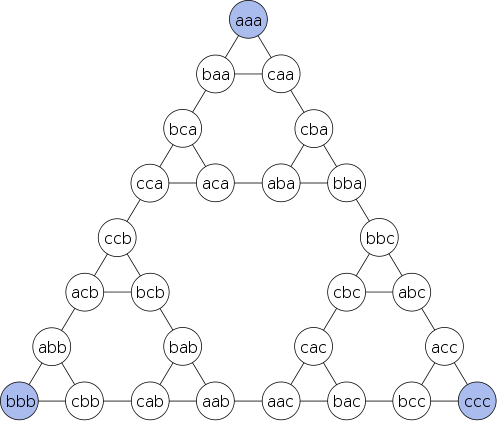
\includegraphics[width=0.7\textwidth]{img/hanoi_graph}
  \end{center}
  {\smaller Image created by nonenmac}
\end{frame}

\begin{frame}
  \frametitle{Explaining the Tower of Hanoi Data Structure}
  \begin{columns}[c]
    \column{0.7\textwidth}
    \begin{itemize}
    \item Each node identifies an state in the problem;
    \item Each character in the string represents one disk and its
      position;
    \item We can have at most 3 state transitions at each state (can
      you prove it?)
    \item To solve the Towers of Hanoi problem, we find the path
      between the start and end states.
    \item (just beware of state explosion)
    \end{itemize}
    \column{0.3\textwidth}    
    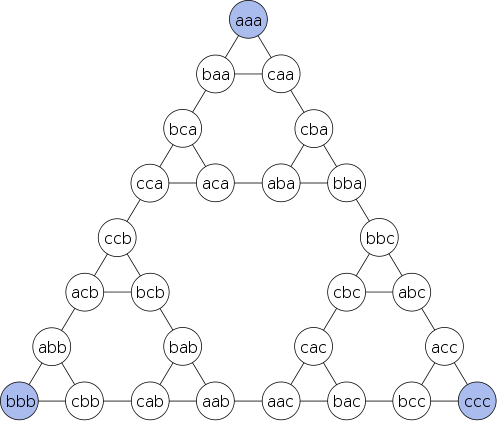
\includegraphics[width=0.9\textwidth]{img/hanoi_graph}
    \vfill
  \end{columns}
\end{frame}

\subsection{Data Structure Library}

%% TODO: Improve this section
\begin{frame}
  \frametitle{Know your data structures!}
  \begin{block}{}
    To be able to do data structure tricks, we need to be familiar
    with a variety of data structures.
  \end{block}

  \bigskip

  \begin{itemize}
  \item What is the time and memory efficiency of each data structure?
  \item What is \structure{programming efficiency} of each data structure?
  \item What are the common uses?
  \item What are the common bugs?
  \end{itemize}
  
\end{frame}

\begin{frame}
  \frametitle{Data Structure Libraries}

  The ``Library'' word can have many meanings:

  \begin{block}{Language Library}
    \begin{itemize}
    \item What function is used to create a dictionary?
    \item What parameters are passed in this function?
    \end{itemize}
  \end{block}

  \begin{block}{Personal Library}
    \begin{itemize}
    \item How many data structures do you personally remember?
    \item Notes on paper can be very useful!
    \end{itemize}
  \end{block}
\end{frame}

\begin{frame}
  \frametitle{Low Level Data Structures}
  \begin{itemize}
  \item Array
    \vspace{.5cm}
  \item Linked List
  \end{itemize}
  
  \bigskip

  \begin{block}{}
    The Array is usually simpler, and less bug prone. But be careful with
    index overflows!
    \medskip
    
    When in doubt, use a bigger array!
  \end{block}
\end{frame}

\begin{frame}
  \frametitle{Medium Level Data Structures}
  \begin{itemize}
  \item Stack
    \vspace{.5cm}
  \item Queue
  \end{itemize}

  \bigskip

  \begin{block}{}
    The stack is the simplest ``complex'' data structure. It is
    implemented with an array and an index.
    \medskip
    
    How do you implement a Queue using two stacks?
    \medskip

    Queue and Stack are used very often.
  \end{block}
\end{frame}

\begin{frame}
  \frametitle{High level data structures}
  \begin{itemize}
  \item Sets
  \item Dictionaries
  \item Priority Queues
  \end{itemize}
  
  \bigskip

  \begin{block}{}
    These structures attach extra information to data: Key,
    Uniqueness, order.
    \medskip

    Try to think of them as combinations of the above techniques. How
    would you implement them?
  \end{block}
\end{frame}

\begin{frame}
  \frametitle{Other data structures}
  \begin{itemize}
  \item Trees
  \item Graphs
  \end{itemize}

  \bigskip

  We well talk about these in future classes
\end{frame}

\subsection{Strings}

\begin{frame}
  \frametitle{String Representation in Computers} 
  When you tyle ``\emph{ls}'', why do numbers appear before letters?

  \bigskip
  
  \begin{block}{}
    Strings in a computer system are represented as an
    \structure{Array of characters}, and each character is represented
    as an index.
  \end{block}
\end{frame}

\begin{frame}
  \frametitle{Characters as numerical indexes: what are the consequences?}
  \begin{itemize}
  \item Operation on characters (Addition, comparison);
  \item Arbitrary order of glyphs;
  \end{itemize}
\end{frame}

\begin{frame}
  \frametitle{Encodings}
  \begin{block}{}
    Encodings are mappings between a set of indexes and a set of
    glyphs. Different encodings cause Mojibake.
  \end{block}

  \medskip

  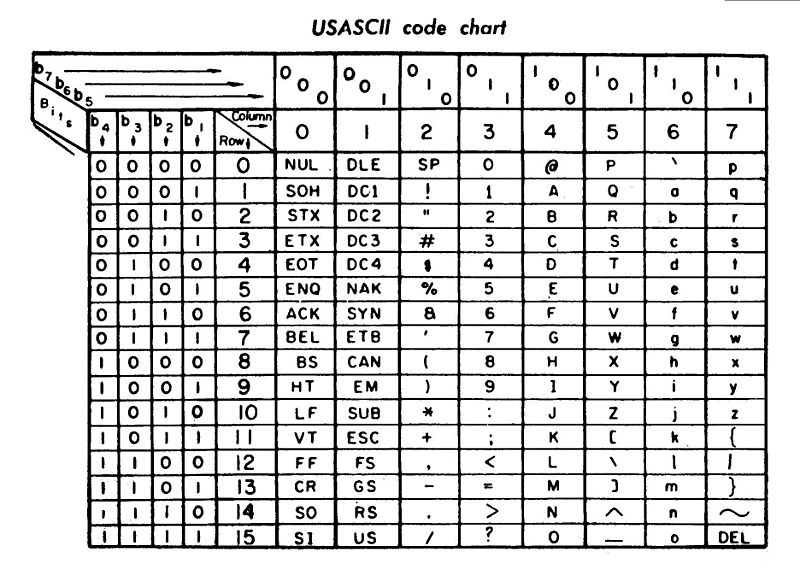
\includegraphics[width=0.7\textwidth]{img/ASCIItableOld}

  \medskip

  ASCII Indexes were selected with very specific properties.
  
\end{frame}

%%%%%%%%%%%%%%%%%%

\section{Closing Points}
\subsection{Closing Points}
\begin{frame}
  \frametitle{This week's problems}
  \begin{block}{List of Problems}
    \begin{itemize}
    \item The 3n+1 Problem
    \item Check the Check
    \item Erdos Numbers
    \item Contest Scoreboard
    \end{itemize}
  \end{block}
  \medskip
  Let's give a quick look on each problem
\end{frame}

\begin{frame}
  \frametitle{For the rest of the week:}
  \begin{itemize}
  \item Next class: Bring your solutions and questions!
    \vfill
  \item Submission deadline is 04-19 23:59:59 (Sunday)
    \vfill
  \item Have a nice week!
  \end{itemize}
\end{frame}


% TODO: Complete Friday Class (by friday)
\section{Friday}
\subsection{Friday Class}
\begin{frame}
  \begin{center}
  {\bf Welcome to Friday Class!}
  \end{center}
\end{frame}

\begin{frame}
  \begin{alertblock}{Important Question}
    Did everyone register in the ``Programming Challenges'' website?
  \end{alertblock}
  
  \bigskip

 You cannot grade without registering!
\end{frame}

\begin{frame}
  \frametitle{Results So far}
  \begin{itemize}
  \item The 3n+1 Problem -- Solved: 24/45
  \item Check the Check -- Solved: 8/45
  \item Erdos Numbers -- Solved: 1/45
  \item Contest Scoreboard -- Solved: 2/45
  \end{itemize}

  \bigskip

  90\% of students who tried solved. But half have not tried yet. Be careful!!

\end{frame}

\begin{frame}
  \frametitle{A few more results}
  \begin{block}{The 3n+1 Problem}
    \begin{itemize}
    \item Average number of tries before succeeding: 8
      \vspace{.5cm}
    \item Maximum number of tries: 57 
      \\\structure{Thanks for the effort!!}
      \vspace{.5cm}
    \item One very fun submission:
    \end{itemize}
  \end{block}
\end{frame}

\begin{frame}
  \frametitle{New Input and Output data}
  \begin{itemize}
  \item Some people had problems with the lack of input data.
    \vspace{.5cm}
  \item Remember that in many problems, you have many ``scenarios'' in
    the same input.
    \vspace{.5cm}
  \item I have added some extra data input for ``Erdos Numbers'' and
    ``Contest Scoreboard''
  \end{itemize}
\end{frame}

\begin{frame}
  \frametitle{New Input and Output data}
  \begin{itemize}
  \item You can also generate your own test cases using the website:
    \url{http://www.udebug.com/}
    \vspace{.5cm}
  \item Access the site and select the problem
    \vspace{.5cm}
  \item Enter the input case, and receive a correct output
    \vspace{.5cm}
  \item Try hard inputs!
  \end{itemize}
\end{frame}

\begin{frame}
  \frametitle{Discussing the Problems}
  \begin{itemize}
  \item Many people have tried the problems in order, don't do this!
    \vspace{.5cm}
  \item Compile problems with C: use strict C, or switch to C++!
    \vspace{.5cm}
  \item Other questions?
  \end{itemize}
\end{frame}

\begin{frame}
  \frametitle{Reviewing the problems}
  \begin{itemize}
  \item The 3n+1 Problem (memory, trap)
  \item Check the Check (bothersome, reverse)
  \item Erdos Numbers (bothersome, structure)
  \item Contest Scoreboard (structure)
  \end{itemize}
\end{frame}

%if ( n % 2 == 0 ) {
%		int div = n & (-n);
%		return sequence(n / div) + bitLength(div) - 1;
%	}else {
%		return sequence((n * 3) + 1) + 1;
%	}

\begin{frame}
  \frametitle{Solving some problems}
  \begin{itemize}
  \item Contest Scoreboard
  \item The Trip
  \item Erdos Numbers
  \end{itemize}
\end{frame}

\begin{frame}
  \frametitle{Extra Announcements I}
  \begin{block}{ICPC International Collegiate Programming Contest}
    \begin{itemize}
    \item Contest day: 6/23 (16:00 - 19:30)
    \item Application deadline: 6/12
    \item ICPC site: \url{http://icpc.iisf.or.jp/}
    \item TPC site: \url{http://conclave.cs.tsukuba.ac.jp/tpc}
    \end{itemize}
  \end{block}
\end{frame}

\begin{frame}
  \frametitle{Extra Announcements II}
  \begin{block}{Ludum Dare}
    \begin{itemize}
    \item Online game making festival
    \item Get feedback from other game makers
    \item Ludum Dare site: \url{http://ludumdare.com/compo/}
    \end{itemize}
  \end{block}
\end{frame}

\begin{frame}
  \begin{center}
    {\bf The end! Ask me anything!}\\
    New problems uploaded tonight
  \end{center}
\end{frame}

\end{document}
